So far, we have proven that there must exist a trade-off between memory and surprisal, and that this trade-off is optimized when languages have relatively short-term dependencies. In this section we qualitatively illustrate the linguistic predictions of our theoretical results  by reanalyzing the data from \cite{fedzechkina-human-2017}.
This is a miniature artificial language study that showed a bias for dependency locality in production in artificial language learning. 
We will show that, as predicted, the languages which were favored in the artificial language learning experiment are those which optimize the memory--surprisal trade-off. 

\subsection{Background: \citet{fedzechkina-human-2017}}

\citet{fedzechkina-human-2017} conducted a miniature artificial language learning experiment in which participants were exposed to videos describing simple events, paired with sentences in an artificial language of the form Subject--Object--Verb or Object--Subject--Verb, in equal proportion, with free variation between these two word orders. The subject and the object were either simple nouns, or complex noun phrases with modifiers. Participants were trained to produce sentences in response to videos.

Crucially, \citet{fedzechkina-human-2017} set up the experiment such that in all training trials, either the subject and the object were both simple, or they were both complex. Then, after participants were sufficiently skilled in the use of the artificial language, they were asked to produce sentences describing videos with mixed complexity of noun phrases. The possible word orders that could be produced in this mixed-complexity setting are shown in Figure~\ref{tab:artificial}; the orders marked $A$ would create short dependencies, and the orders marked $B$ would create long dependencies. 
\begin{figure}
	\textbf{A Orders: Short Dependencies}

	OSV: [[Adjective Noun Postposition] Noun-\textsc{Case}] Noun Verb

	SOV: [[Adjective Noun Postposition] Noun] Noun-\textsc{Case} Verb

%
%	OSV:
%		\begin{tabular}{ccc}
%%			Object & Subject & Verb \\
%			\fbox{\begin{tabular}{llllll}
%				\fbox{\begin{tabular}{llll} Adjective &Noun &Postposition\end{tabular}} & Noun-\textsc{\textsc{Case}}
%					\end{tabular}} & \fbox{\begin{tabular}{l}Noun\end{tabular}} & \fbox{\begin{tabular}{l}Verb\end{tabular}}  \\
%		\end{tabular}
%\\
%
%SOV:
%		\begin{tabular}{ccc}
%			%			Subject & Object & Verb \\
%			\fbox{\begin{tabular}{llllll}
%				\fbox{\begin{tabular}{llll} Adjective &Noun &Postposition\end{tabular}} & Noun
%					\end{tabular}} & \fbox{\begin{tabular}{l}Noun-\textsc{\textsc{Case}}\end{tabular}} & Verb \\
%		\end{tabular}
%\\
%\\

	\textbf{B Orders: Long Dependencies}

	SOV: Noun [[Adjective Noun Postposition] Noun-\textsc{Case}] Verb

	OSV: Noun-\textsc{Case} [[Adjective Noun Postposition] Noun] Verb
%
%		\begin{tabular}{ccc}
%%			Subject & Object & Verb \\
%			 \fbox{\begin{tabular}{l}Noun\end{tabular}} &  \fbox{\begin{tabular}{llllll}
%				\fbox{\begin{tabular}{llll} Adjective &Noun &Postposition\end{tabular}} & Noun-Case
%		\end{tabular}}  &  \fbox{\begin{tabular}{l}Verb\end{tabular}}  \\
%		\end{tabular}
%\\
%		\begin{tabular}{ccc}
%%			Object & Subject & Verb \\
%			\fbox{\begin{tabular}{l}Noun-Case\end{tabular}} & \fbox{\begin{tabular}{llllll}
%				\fbox{\begin{tabular}{llll} Adjective &Noun &Postposition\end{tabular}} & Noun
%		\end{tabular}} & Verb \\
%		\end{tabular}
%
			\caption{Production targets in the miniature artificial language from \cite{fedzechkina-human-2017}. The language has head-final order, with free variation between SO and OS orders. When one of the arguments is much longer than the other, placing the longer one first ($A$ orders) shortens syntactic dependencies, compared to $B$ orders.}\label{tab:artificial}

\end{figure}

\citet{fedzechkina-human-2017} found that participants favored the $A$ orders over the $B$ orders, despite the fact that there was no pattern in the participants' training input which would have favored $A$ over $B$. That is, when exposed to input which was ambiguous with respect to language $A$ or $B$, participants favored language $A$. \citet{fedzechkina-human-2017} explained this result in terms of dependency locality: because the $A$ orders create short dependencies between the verb and its arguments and the $B$ orders create long dependencies, participants preferred the $A$ orders.

\subsection{Calculating the memory--surprisal trade-off for the artificial languages}

The Efficienct Tradeoff Hypothesis predicts that the favored language $A$ has a steeper memory--surprisal trade-off curve than the disfavored language $B$. Because of the controlled nature of this artificial language, we are able to test this hypothesis by exactly computing the bound on memory as given in Theorem~\ref{prop:suboptimal}. In fact, for this toy process, we can prove that the bound provided by the theorem is achievable, meaning that our computations reflect the true memory--surprisal trade-off curve, and not only a lower bound on it.

We only consider the head-final version of \citet{fedzechkina-human-2017}'s artificial language. This is because our bound on the memory--surprisal trade-off curve is invariant under reversal of a language. That is, if we take a language and reverse the order of all the words in all its sentences, we would measure the same lower bound on the memory--surprisal trade-off curve (for a proof, see SI Section \REF). Therefore, strictly head-final and strictly head-initial languages are equivalent under our bound.\footnote{Note that this invariance to reversal applies only to our \emph{lower bound} on the memory-surprisal trade-off curve; the true curve is not generally invariant to word order reversal \citep{crutchfield-times-2009}.} 

%The language has consistent head-final order, and uses case marking on objects.
%The relevant production targets are transitive sentences where one of the two arguments is much longer than the other, due to the presence of a PP modifier, as shown in Table~\ref{tab:artificial}.
%The language has variable order of subjects and objects; for the production targets, the B versions produce much longer dependencies than the A versions.
%Dependency Length Minimization thus predicts that speakers are more likely to use the A versions.
%\cite{fedzechkina-human-2017} confirmed this experimentally.

We constructed a stochastic process representing the language consisting of sentences with the $A$ orders from Figure~\ref{tab:artificial}, and one language consisting of the $B$ orders. Following the experimental setup of \cite{fedzechkina-human-2017}, we assigned equal probability to the two possible configurations per language, and used a separate set of nouns (inanimate nouns) for the embedded noun in the long phrase.

% TODO: Does the process only include those orders, or does it also include the SOV and OSV orders with equal-complexity O and S?

We interpreted each of the two languages as a stationary processes, extending infinitely in both directions, by concatenating independent samples drawn from the language.
We computed the bounds on memory and surprisal (\ref{eq:memory-bound}-\ref{eq:surprisal-bound}) from Theorem~\ref{prop:suboptimal} from a chain of 1000 independently sampled sentences, for each of the two versions of the toy language.
% TODO: More on how this was done.			
% TODO: Convert nats to bits

\subsection{Results}	

\begin{figure*}
\centering
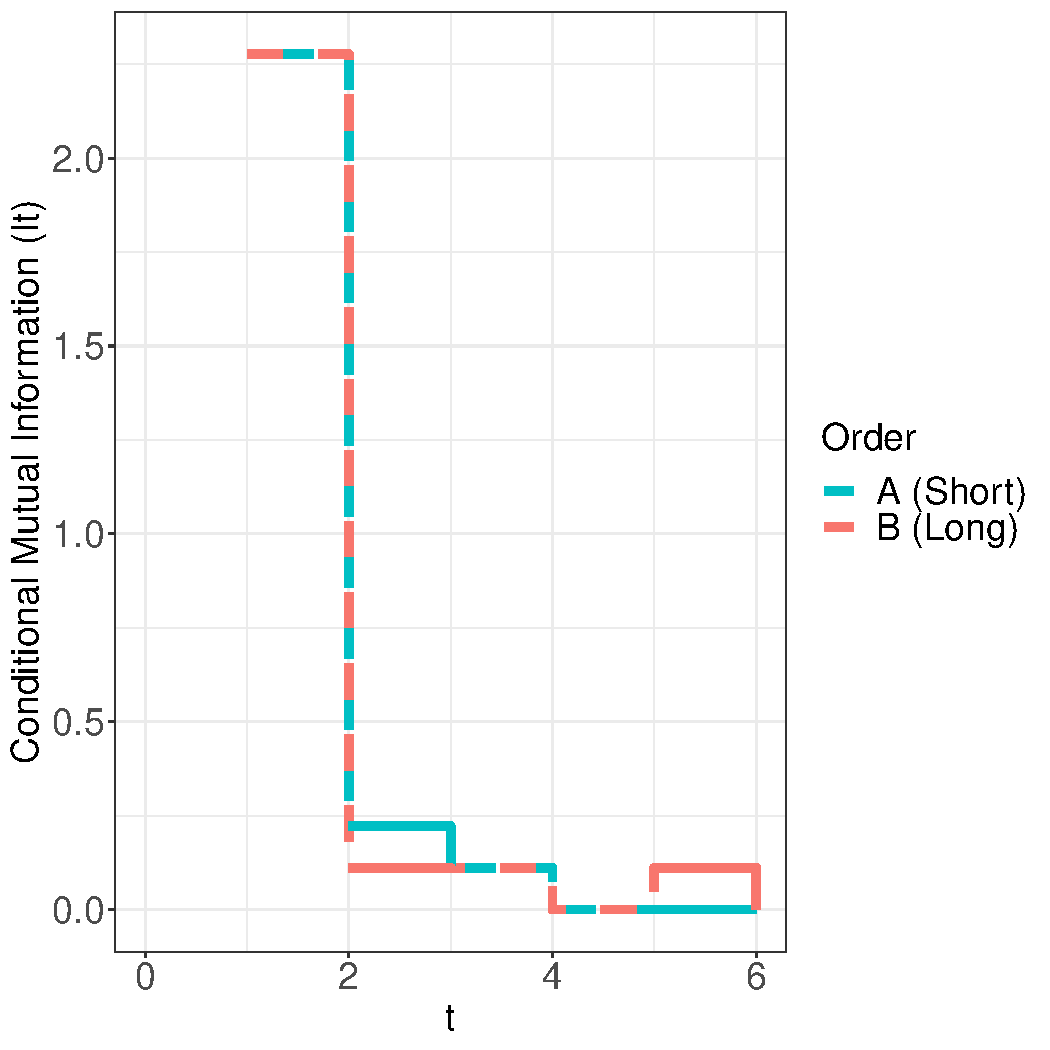
\includegraphics[width=0.45\textwidth]{figures/toy-mis.pdf}
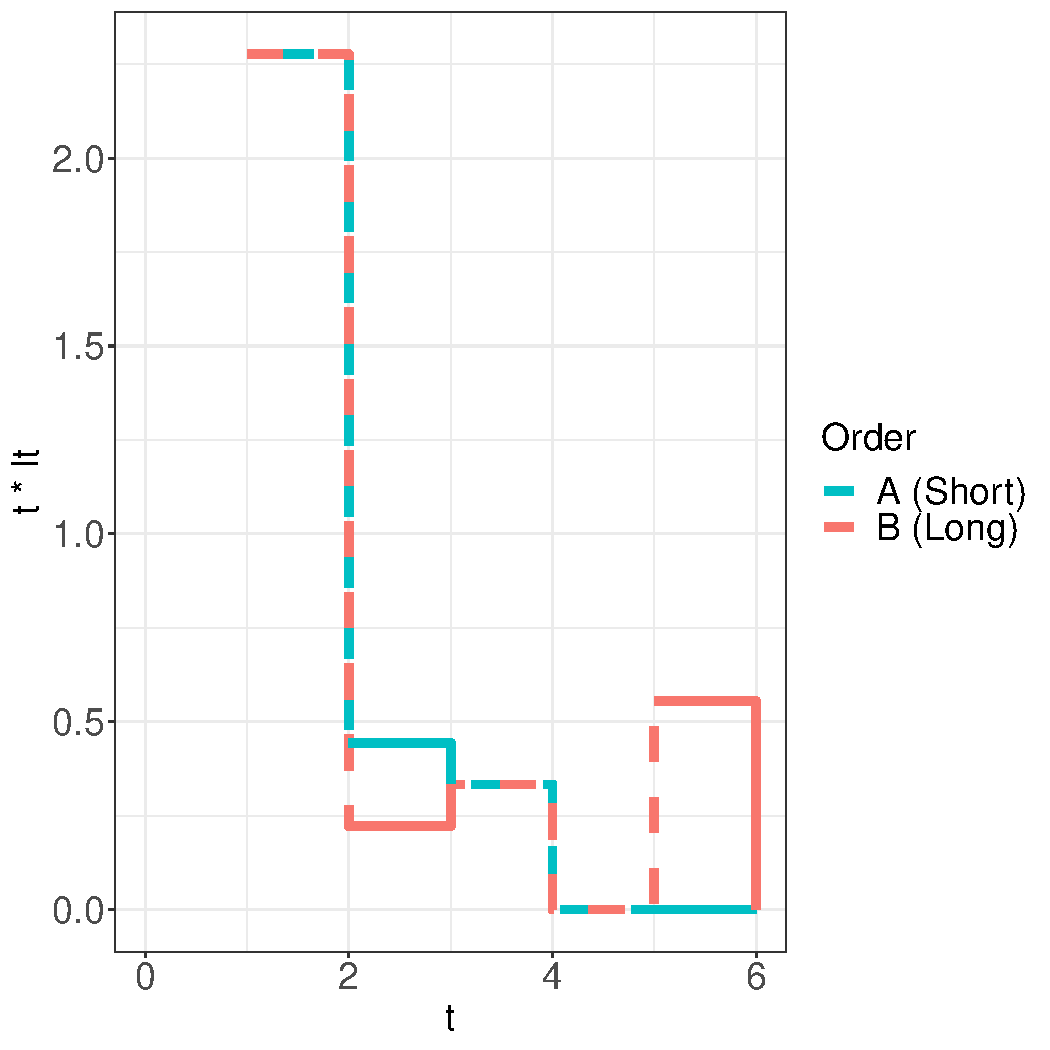
\includegraphics[width=0.45\textwidth]{figures/toy-t-mis.pdf}
%
	\caption{Left: Decay of conditional mutual information $I_t$, as a function of the distance $t$, for the two versions in the artificial language. The areas under the two curves are identical, corresponding to the fact that both orders are equally predictable. However, mutual information decays faster in language $A$.\ \ \ Right: The minimal memory requirement $t I_t$ to store $I_t$ bits of information for timespan $t$, as a function of $t$. The area under the $B$ curve is larger, corresponding to larger memory demand for this order.}\label{fig:toy-mis}
\end{figure*}

Figure~\ref{fig:toy-mis} (left) shows the curve of the conditional mutual information $I_t$ as a function of the distance $t$, for the two languages $A$ and $B$. 
The curves differ at $t=2$ and $t=5$: 
About 0.073 units of predictive information that are at distance $t=2$ in the $A$ orders are moved to $t=5$ in the $B$ orders.
The source of the difference lies in predicting the presence and absence of a case marker on the second argument---i.e., whether to anticipate a subject or object.
In the $A$ orders, considering the last two words is sufficient to make this decision.
In the $B$ orders, it is necessary to consider the word before the long second constituent, which is five words in the past.

The total amount of predictive information---corresponding to the area under the $I_t$ curve----is the same for both languages, indicating that both languages are equally predictable. However, the memory demands differ between the two languages. Figure~\ref{fig:toy-mis} (right) shows the minimal memory requirements for remembering predictive information at a distance $t$ ($t\cdot I_t$) as a function of $t$. As $I_t$ decays faster in $A$ orders, the total area under the curve differs between $A$ and $B$, and is larger in $B$. Thus, achieving the same predictive accuracy in language $B$ requires more memory resources than in language $A$.
			%This area corresponds to the lower bound in (\ref{eq:memory-bound}), and is 2.21 nats in A orders, and 2.43 nats in B orders.

%While (\ref{eq:memory-bound}) is a general lower bound, it can be proven that this bound is actually tight in the case of this specific example.\footnote{This can be shown by computing the causal states and then showing that the crypticity is zero, both of which is tractable in the case of this small-scale artificial language.}
%That is, a speaker who optimally allocates memory resources will spend 2.21 nats in A orders, and 2.43 nats in B orders.

\begin{figure}
\centering
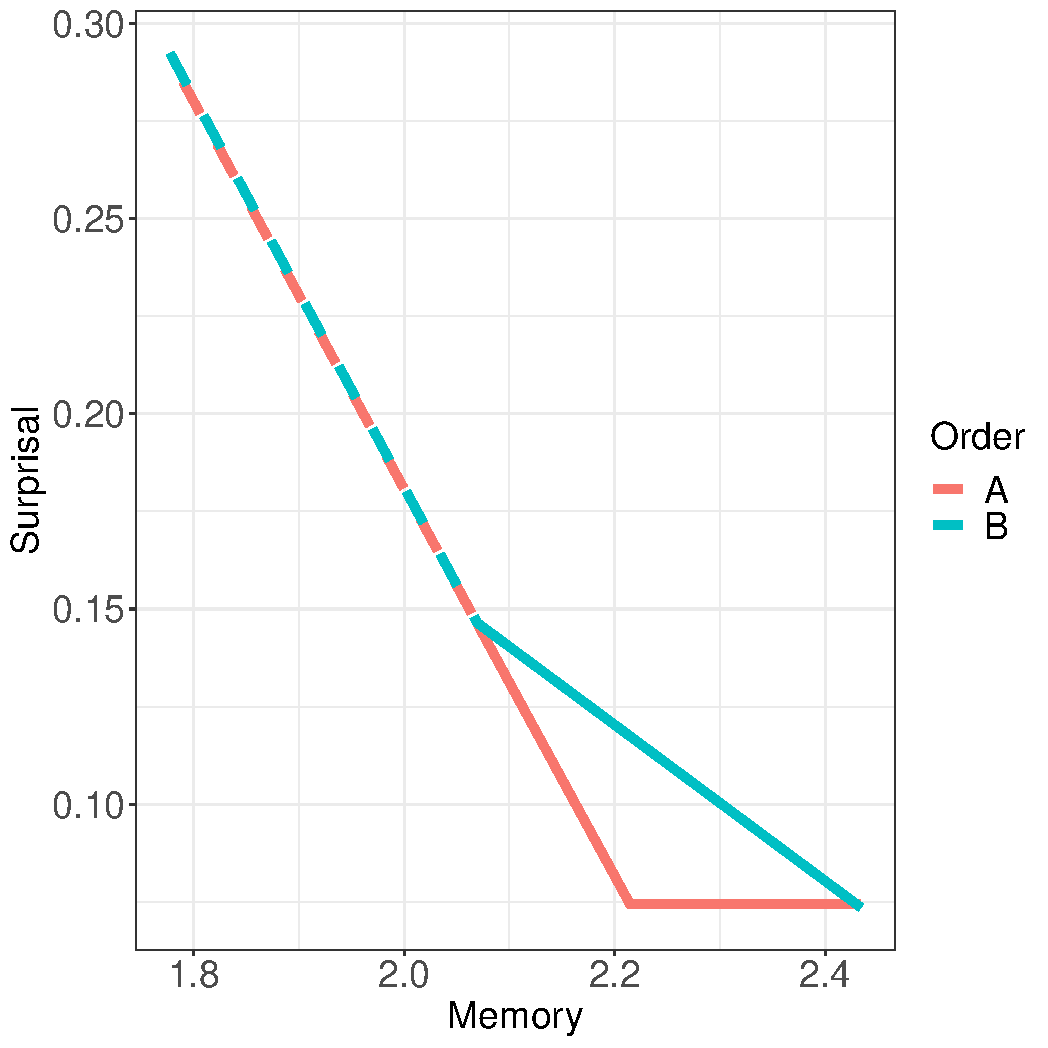
\includegraphics[width=0.45\textwidth]{figures/toy-mem-surp.pdf}
	\caption{Tradeoff between listener memory and surprisal for the two versions of the artificial language from \cite{fedzechkina-human-2017}. Language $A$ requires less memory at the same level of surprisal. }
	\label{fig:toy-listener-tradeoff}
\end{figure}

Figure~\ref{fig:toy-listener-tradeoff} shows the resulting memory--surprisal trade-off curve for the two versions of the artificial language from \cite{fedzechkina-human-2017}, obtained by tracing out all values of $T=1, 2, \dots$ in the theorem, and connecting the points linearly.\footnote{Linear interpolation is justified because rate-distortion curves such as the memory-surprisal tradeoff curve are convex \citep{berger2003rate}.}
The curve shows that, at any desired level of surprisal, language $A$ requires at most as much memory as language $B$.
To reach optimal surprisal, the empirically-favored language $A$ requires strictly less memory.


%It is important to stress that, even though we computed this value by considering the number of words impacting predictions at a given point in time, this bound holds independently of the actual implementation and architecture of memory and predictions.





%Both languages have the same overall entropy rate, but they differ in the distribution of predictive information.
%
%plot of $I_t$
%
%The areas under the curves are identical.
%
%good version
%
%%CONTEXT LENGTH 0   2.06856758681  9997.93143241   0.0
%%CONTEXT LENGTH 1   0.29195106479  1.77661652202   1.77661652202
%%CONTEXT LENGTH 2   0.0729865489103  0.21896451588   2.21454555377
%%CONTEXT LENGTH 3   0.0729865489103  0.0   2.21454555377
%%CONTEXT LENGTH 4   0.0729865489103  0.0   2.21454555377
%%CONTEXT LENGTH 5   0.0729865489103  0.0   2.21454555377
%%CONTEXT LENGTH 6   0.0729865489103  0.0   2.21454555377
%
%bad version
%
%%CONTEXT LENGTH 0   2.06937301571  9997.93062698   0.0
%%CONTEXT LENGTH 1   0.291673373027  1.77769964269   1.77769964269
%%CONTEXT LENGTH 2   0.145830550934  0.145842822093   2.06938528687
%%CONTEXT LENGTH 3   0.145830550934  0.0   2.06938528687
%%CONTEXT LENGTH 4   0.145830550934  0.0   2.06938528687
%%CONTEXT LENGTH 5   0.0729152754672  0.0729152754672   2.43396166421
%%CONTEXT LENGTH 6   0.0729152754672  0.0   2.43396166421
%%CONTEXT LENGTH 7   0.0729152754672  0.0   2.43396166421
%%
%
%
%
%%
%%grammar:
%%
%%S $\rightarrow$ Obj Subj V (1/2) | Subj Obj V (1/2)
%%
%%Obj $\rightarrow$ NP di
%%
%%Subj $\rightarrow$ NP
%%
%%NP $\rightarrow$ N (3/4) | PP NP (1/8) | Adj NP (1/8)
%%
%%PP $\rightarrow$ NP P
%%
%
%




\subsection{Discussion}

In a reinterpretation of previous experimental findings, we showed that the languages which are favored in an artificial language learning experiment are those which optimize the memory--surprisal trade-off.
%\jd{i'm not sure that saying it quite this generally is justified, given that this is a reanalysis of just one dataset. maybe tone down slightly and/or say that it would be useful to do this kind of analysis on additional, similar datasets -- the prediction, in any case, is clear.}
This is evidence that learners and/or speakers have a bias toward word orders that optimize the trade-off. 
Furthermore, this result solidifies the link between the memory--surprisal trade-off and more traditional notions from linguistics, such as dependency locality. 
We found that the word orders which are optimal from the perspective of dependency locality are also those orders which are optimal from the perspective of the memory--surprisal trade-off, in the setting of a small controlled artificial language.
In Study 2, we scale this approach up to larger corpora of real text.
%\jd{again, just within one small toy dataset. i'd acknowledge that here, then you have a nice segue to the next section}.
